\graphicspath{{content/chapters/literature_review/discussion/figures}}

\section{Discussion}
\label{sec:literature_review_discussion}

This section will give a retrospective of all that was explored in the reviewed literature, starting from the computer vision tasks tackled, the problems that arose, and how they approached them with possible solutions.

\subsection{Computer Vision Tasks}
\label{subsec:discussion_computer_vision_tasks}

\begin{table}[]
\captionsource(Models against visual datasets){Which models were trained and tested against which datasets.\label{tab:models_against_datasets}}{Written for this dissertation}
\begin{threeparttable}
    \begin{tabular}{@{}rcccccc@{}}
        \toprule
                    & SHAPES & VQA          & CLEVR & GQA & VCR & VisDial \\ \midrule
        NMN      & Yes    & Yes          & No    & No  & No  & No      \\
        N2NMN    & Yes    & Yes          & Yes   & No  & No  & No      \\
        SNMN     & No     & Yes          & Yes   & No  & No\tnote{1} & No      \\
        NMNs\pm\tnote{2}    & No     & No           & No    & No  & No  & No      \\
        DPNMN    & No     & No           & Yes   & No  & No  & No      \\
        MAC      & No     & Yes\tnote{3} & Yes   & Yes & No  & No      \\
        LNMN     & No     & No           & Yes   & No  & No  & No      \\
        MMN      & No     & No           & Yes   & Yes & No  & No      \\
        R2C      & No     & No           & No    & No  & Yes & No      \\
        CorefNMN & No     & No           & No    & No  & No  & Yes     \\
        NMNVD    & No     & No           & No    & No  & No  & Yes     \\ \bottomrule
    \end{tabular}
    \begin{tablenotes}
        \item[1] This will be implemented and tested in this dissertation.
        \item[2] Was only developed and tested on a bespoke dataset\cite{chen_teaching_2022}.
        \item[3] Tested and evaluated on v1.0 of the dataset\cite{hudson_compositional_2018}.
    \end{tablenotes}
\end{threeparttable}
\end{table}

\gls{vqa} is the first task discussed and the simplest in structure and challenge; one image, one question, and one required answer which can be open-ended or multi-label.
Of the reviewed datasets, it has the largest coverage \cite{andreas_deep_2016,agrawal_vqa_2016,johnson_clevr_2016,hudson_gqa_2019} with the CLEVR dataset having the greatest testing coverage among \gls{nmn}-based models\cite{fishandi_neural_2023}.
This would make sense as the dataset, while using synthetic images, prioritises highly-compositional questions which require multiple reasoning steps to predict an answer, similar to \gls{gqa}.

\gls{vcr} is the next discussed task type to be formalised\cite{zellers_recognition_2019}.
This task extends \gls{vqa} by using realistic images taken from still video frames, omitting knowledge mostly found in the moments leading up to the taken image.
Through this method, models will need to focus on inferring knowledge either from commonsense knowledge or from finer details in the image.
Unlike \gls{vqa}, the \gls{vcr} dataset\cite{zellers_recognition_2019} is one of the only few datasets present for this task type due to its recent introduction, with the \gls{r2c} model discussed being one of the models trained and tested on the dataset.
\todo[inline]{GD-VCR exists which is a more geo-diverse-focused variant of the dataset meant to target commonsense knowledge about different cultures. Should this be introduced?}

\gls{vd} is the last task type of these three to be introduced and formalised\cite{das_visual_2019}.
It follows a more human dialogue-like flow where each image is paired with a caption and question-answers pairs provided as data to the model.
The questions and answers build context around the image which offer a stricter benchmark on visual comprehension for compositional models such as \gls{nmn}.
Similar to \gls{vcr}, the VisDial dataset is one of the only datasets which present this task type \cite{das_visual_2019}.
\todo[inline]{CLEVR-Dialog was recently published which uses CLEVR images. Should this be introduced?}

Despite being task types with different data layouts and amounts of input data, they all share the same goal of providing answers to questions which are grounded in images.
The main difference between the tasks is in how each of their datasets tackle the various pitfalls and challenges of answering these questions.
CLEVR, SHAPES, and GQA, all primarily focus on the compositionality of their questions with a focus on how compositional models perform reasoning steps to get to the correct answer\cite{andreas_neural_2016,johnson_clevr_2016,hudson_gqa_2019}.
\gls{vqa}, \gls{vcr}, \gls{gqa}, and VisDial all use natural or realistic images instead of synthetic computer-generated images, arguing that since these better mimic real-life scenarios, they would allow a model to adopt more robust reasoning\cite{agrawal_vqa_2016,hudson_gqa_2019,zellers_recognition_2019,das_visual_2019}.
One experiment by \cite{sejnova_compositional_2018} --- where an \gls{n2nmn}-based model was trained on CLEVR and then tested on both the CLEVR test set and a custom dataset of CLEVR-like realistic images --- found the model had no consistency in both accuracy between both test sets and between multiple questions around the same image \cite{sejnova_compositional_2018}.
They also concluded that further experiments and analysis on the pretraining of models on virtual datasets would need to be carried out before determining if virtual datasets would be viable for real-world applications or not, and just how much of an impact real-world variables such as lighting and noise affect model predictions \cite{sejnova_compositional_2018}.

\subsection{Modules of the NMN Models}
\label{subsec:modules_of_the_nmn_models}

Now that the vision/language tasks have been discussed, the approaches that each model takes to solving the tasks in a compositional manner will be explored.

Marked as the first major step for solving a task, the model must first determine the layout of neural modules, parameters to be passed between these modules, and which module instances to activate.
This challenge is known as \glsfirst{nas}, and is the task of model finding a suitable model architecture across a search space of possible architectures (as seen in Figure~\ref{fig:neural_architecture_search_overview})\cite{elsken_neural_2019}.
The architecture chosen is the one most likely to provide the highest prediction/performance for the given model input when executed.
This plays a core part in \gls{nmn} models and is explored in Table~\ref{tab:models_module_inventory} since having high-performant modules would not make for good predictions without the proper layout and input parameters.
Based on the models reviewed, most appear to employ discrete (D) architecture selection either based on rule-based parsing \cite{andreas_neural_2016,chen_meta_2020} or with a \gls{s2s} \gls{rnn} to generate the layout \cite{hu_learning_2017,chen_teaching_2022,su_toward_2020,kottur_visual_2018,cho_visual_2021}.
On the other end, some models employ a non-discrete (ND) soft layout selection, all of which use a \gls{bilstm} cell to generate module weights and text attention using the given input text embeddings \cite{hu_explainable_2019,hudson_compositional_2018,pahuja_learning_2019}.

Following the layout selection are the actual modules.
Each model has an inventory defined by several neural module types which are dedicated to specific tasks such as finding objects or comparing, etc.
Most of the models discussed have specific, hand-designed module types (S) that are designed to learn best at specific tasks \cite{andreas_deep_2016,hu_learning_2017,hu_explainable_2019,chen_teaching_2022,su_toward_2020,kottur_visual_2018,cho_visual_2021}.
Most models with specific types share a very similar inventory with modules such as finding objects, relocate attention, combine attentions, etc.
Some models implement additional module types for even more specific use-cases such as arithmetic tasks \cite{chen_teaching_2022} or for performing visual coreference resolution \cite[text]{kottur_visual_2018,cho_visual_2021} (see chapters ~\ref{subsec:coreference_neural_module_network} and ~\ref{subsec:neural_module_network_for_visual_dialog}).
There are some models however, which employ an inventory of generic module types (G) that the model must learn itself what models it should create and use for solving the tasks for which it's being trained \cite{hudson_compositional_2018,pahuja_learning_2019,chen_meta_2020}.
While the implementations vary across models, they generally posess some form of memory, inputs for at least one attention or more, a general-purpose unit which combines its memory and attention inputs to produce an output, and (optionally) an answering unit for producing the final outputs that the model will convert to an answer prediction.

\begin{figure}[htbp]
    \centering
    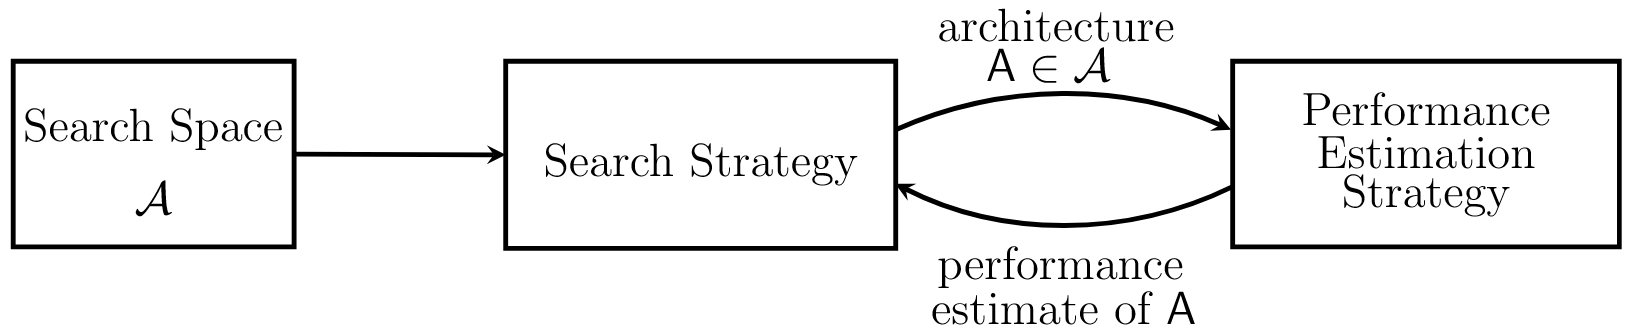
\includegraphics[width=\textwidth,keepaspectratio]{content/chapters/literature_review/discussion/figures/neural_architecture_search_overview.png}
    \captionsource(\acrshort{nas} overview){An abstract overview of the \acrshort{nas} task showing how a search strategy chooses the architecture for a search space and how to preemptively filter architectures that obviously wouldn't be suitable using \acrshort{pes}.\label{fig:neural_architecture_search_overview}}{\citeauthor{elsken_neural_2019}\cite{elsken_neural_2019}}
\end{figure}

\todo[inline]{Discuss in further detail how these other models expand upon the \gls{nmn}, major/minor architecture differences, and the tasks or challenges they target.}

\begin{table}[]
\begin{tabularx}{\linewidth}{cXcXc}
    \toprule
    \multicolumn{5}{c}{VQA/VD Models} \\ \midrule
    Model & \gls{nas} approach & Modules & Type  \\
    NMN & Rule-based parsing (see Chapter ~\ref{subsec:neural_module_network}). & D & find, transform, combine, describe, measure & S  \\
    N2NMN & Seq2Seq RNN (See Chapter ~\ref{subsec:n2nmn}). & D & find, relocate, and, or, filter, count, exist, describe, less, more, equal, compare & S  \\
    SNMN & \gls{bilstm}-generated module weights with txt attention (See Chapter ~\ref{subsec:stack_neural_module_network}). & ND & find, transform, and, or, filter, scene, answer, compare, noOp & S  \\
    NMNs\pm & Similar to N2NMN with type-constrained grammar\cite{gupta_answering_2020}. & D & find, filter, relocate, find-num, find-date, count, compare-num-lt, time-diff, find-max-num, span, compare-date, add, sub & S  \\
    DPNMN & Similar to N2NMN with an RPN for spatial information. & D & find, relocate, and, or, describe, compare & S  \\
    MAC & \gls{bilstm} and fixed-length cell array where each cell can 'skip' itself and relay input to the next cell. & ND & MAC cells & G  \\
    LNMN & Similar to SNMN & ND & General modules (Expand further). & G  \\
    MMN & Rule-based parser feeding into a coarse-to-fine program generator. & D & Meta modules & G  \\
    CorefNMN & Similar to N2NMN but augmented with a memory network for attention-over-text. & D & find, relocate, and, or, filter, count, exist, describe, less, more, equal, compare, not, refer, exclude & S  \\
    NMNVD & Similar to CorefNMN. & D & find, relocate, and, refer, describe, compare & S  \\ \bottomrule
\end{tabularx}
\captionsource(Models module inventory)
    {A full breakdown of the model inventory and layout construction architecture of each model discussed. Selection denotes whether the module selection of a model is a soft selection (ND) --- and thus trainable with back-propagation --- or fully discrete (D) and instead requires an alternate learning strategy such as reinforcement learning. The Type specifies whether the modules listed are Specified (S) in that they have a fixed behaviour and only their weights and biases are learned, or whether they are Generic (G) and are able to learn and apply different behaviours without prior implementation or knowledge.\label{tab:models_module_inventory}}
    {Adapted from \citeauthor{fishandi_neural_2023}\cite{fishandi_neural_2023} with additional model information from models covered in this literature review}
\end{table}
